\section{Background}

\subsection{UPPAAL}



\subsection{Timed automata in UPPAAL}
\begin{definition}[Definition of timed automaton \cite{Alur1990}]
A timed automaton is a tuple $(\Sigma, S, S_0, C, E)$ where:\\
$\Sigma$ - input alphabet;\\
$S$ - finite set of automaton states;\\
$S_0 \subseteq S$ - set of start states; \\
$C$ - finite set of clocks; \\
$E \subseteq S \times S [\Sigma \cup {\epsilon}] \times 2^C \times \Phi(C)$ - set of transitions\\\\
An edge in timed automaton is a tuple $\langle s, s', \sigma, \lambda \delta \rangle$, where:\\
$s$ - origin state;\\
$s`$ - destination state;\\
$\sigma$ - input symbol for the transition;\\
$\lambda$ - set of clocks to be reset with this transition;\\
$\delta$ - condition enabling the transition;\\
\label{def:automaton}
\end{definition}


\subsection{Modeling in UPPAAL}


% Pseudo-code for mutex
\begin{figure}[H]
\caption{Peterson’s mutual exclusion algorithm 
\label{fig:mutex_code}
\cite{SmallTutorial2009}, \cite{Peterson1981}}
\begin{tabular}{|p{0.5\textwidth}|p{0.5\textwidth}|}
\hline
\textbf{Process 1} & \textbf{Process 2} \\
\hline
\begin{lstlisting}[basicstyle=\ttfamily]
req1=1;
turn=2;
while(turn!=1 && req2!=0);
// critical section:
job1();
req1=0;
\end{lstlisting}
&
\begin{lstlisting}[basicstyle=\ttfamily]
req2=1;
turn=1;
while(turn!=2 && req1!=0);
// critical section:
job2();
req2=0;
\end{lstlisting}
\\
\hline
\end{tabular}
\end{figure}


% Mutex implementation in UPPAAL
\begin{figure}[H]
\caption{Mutex automata in UPPAAL \cite{SmallTutorial2009}}
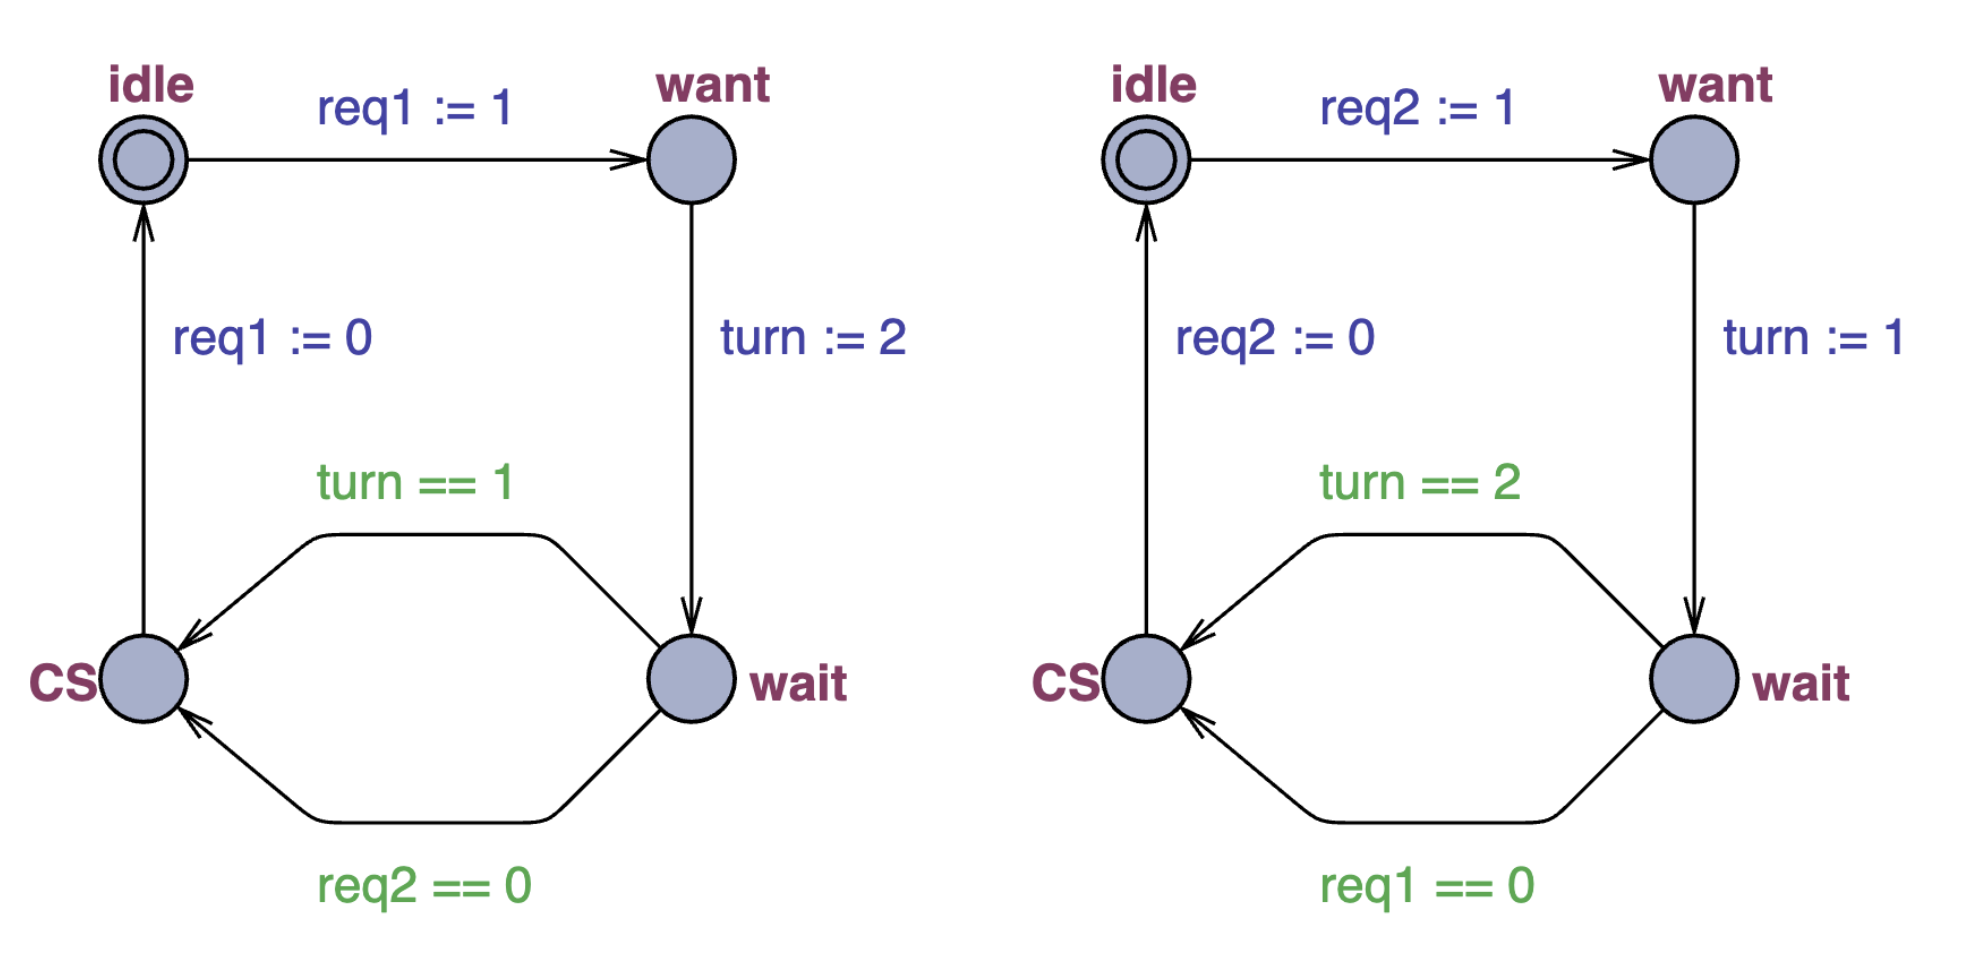
\includegraphics[width=\textwidth]{images/mutex.png}
\label{fig:mutex_uppaal}
\end{figure}



\subsection{Verifying properties in UPPAAL}

% Logical quantifiers in UPPAAL
\begin{definition}[Logical quantifiers in UPPAAL \cite{Bengtsson2004}]
The formulas should be one of the following forms\\
- \texttt{A[]$\phi$} -- Invariantly $\phi$.\\
- \texttt{E<> $\phi$} -- Possibly $\phi$.\\
- \texttt{A<> $\phi$} -- Always Eventually $\phi$.\\
- \texttt{E[] $\phi$} -- Potentially Always $\phi$.\\
- \texttt{$\phi$ --> $\psi$} -- $\phi$ always leads to $\psi$.\\
where $\phi, \psi$ are local properties that can be checked locally on a state, i.e. boolean expressions over predicates on locations and integer variables, and clock constraints.
\label{def:quantifiers}
\end{definition}


% Successfully verified properties for mutex
\begin{figure}[H]
\caption{Successfully verified properties for mutex \cite{SmallTutorial2009}}
\label{fig:mutex_verification}
\begin{lstlisting}[style=code]
A[] not (P1.CS and P2.CS)
E<> P1.CS
E<> P2.CS
\end{lstlisting}    
\end{figure}